\documentclass[../diss.tex]{subfiles}

\begin{document}

This chapter shows that the implementation works as intended through the use of unit tests and custom benchmarks. These benchmarks have been designed to stress the garbage collector in an attempt to expose any faults in the implementation. We will see that unit testing was employed to test each component in isolation before seeing the benchmarks which test the garbage collector as a whole unit. Finally, the performance of the garbage collector is discussed which leads to ideas about future work or alternative design patterns for C programs. I will not be comparing the performance against the Boehm garbage collector, the reasoning behind this is that their solution is a more mature piece of software with many platform-specific enhancements which would be hard to convincingly beat in the given timescale. Appendix \ref{appendix:evaluation} contains source code for the benchmarks, unit tests and Matlab scripts.

\section{Overall Results} \label{sec:overallresults}

% Talk about when the requirements were met and the evidence of it

The success criteria were first outlined in the project proposal (Appendix \ref{appendix:initialproposal}). In the requirements analysis (\cref{sec:requirements}) these were refined into smaller objectives such that an implementation achieving these would also meet the main success criteria.

\begin{enumerate}
    \item Produce a garbage collector which never collects a live object.
    \item The garbage collector should run when the number of objects in a generation passes a threshold or when malloc returns NULL indicating that there isn't enough space on the heap.
    \item  It should collect at least 90\% of garbage each time it is run.
\end{enumerate}
 
All three criteria are of equal importance. I could meet criterion 1 by implementing a garbage collector which never runs or never collects any objects. Therefore, criteria 2 \& 3 are required to ensure the result is useful.

My implementation has met all the success criteria, as shown by the following unit test and benchmark results, and I have implemented an extension which makes the garbage collector thread-safe.

\section{Unit Tests}

Unit tests are a good programming practice when working on large scale projects. Each module was unit tested to ensure correctness and the overall results can be seen in Figure \ref{fig:unittests}. The unit tests for a particular source file can be found under the same name (although with a different extension) in the test directory.

The unit tests use Catch's BDD-style specification which is useful to clearly setup the state before performing the test we are concerned with. My unit tests focus on maintaining data-structure consistency when operations are applied to a particular state.

\begin{figure}[h]
    \centering
    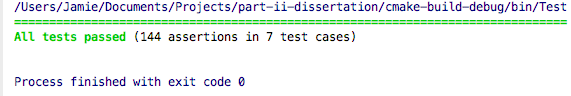
\includegraphics[max width=\linewidth]{figs/unittests.png}
    \caption{A figure showing the result of running the unit tests}
    \label{fig:unittests}
\end{figure}

\section{Benchmarks} \label{sec:benchmarks}

In this section I measure the amount of garbage that is recycled for single and multi-threaded programs. From this evidence I will conclude that the garbage collector has met the success criteria.

I produced two benchmarks that demonstrate key features of the garbage collector. As well as using the two benchmarks I also evaluated against multi-threaded versions of the benchmarks in which the same task is running over many threads. These benchmarks are also unit tested for correctness and their memory statistics are recorded for evaluation. When deallocating memory, the contents are invalidated and set to all 0s. This destroys the original contents of the allocated memory making it likely that freeing a live object will cause an error.

There is a consistent naming convention used throughout the evaluation, benchmarks take the form [Name][$N$]($x$), where Name is the name of the benchmark, $N$ is the number of threads it uses and $x$ is the input.

\subsection{Fib Benchmark}

This benchmark attempts to produce Fibonacci numbers using a naive method. It uses recursion and allocates a new integer for each temporary number. This is clearly not a very good example of real-world programs but it allows me to demonstrate that the garbage collector is running and that it collects at least 90\% of garbage. This benchmark allocates memory which dies very quickly and therefore is good for demonstrating generational algorithm properties. As well as the single-threaded version, I use a multi-threaded version which attempts to compute many Fibonacci numbers at once on 8 threads.

Figure \ref{fig:fib1graph} displays the results for running the single threaded benchmark with a threshold of 200 allocations and calculates the 20th Fibonacci number. From this we can see that garbage is being collected and that the collector is running frequently every 200 allocations. The benchmark completes with the result of 6765 which is the correct result. Table \ref{tab:fib1stats} shows the garbage collector statistics on completion. From these statistics we can see that 98\% of garbage was collected. With longer running tests such as calculating the 30th Fibonacci number, we get 99.99\% of garbage collected although the graphs produced by these are very compact because of the amount of data. With short running programs which do not allocate as much memory, it is possible to get relatively low collection rates. For example computing the 10th Fibonacci number with a threshold of 10 objects gives us a collection rate of 73.4\% ($=80/109$). It is important to note that one object should be live because it contains the result. When I force a garbage collection before the program exits the collection rate improves to 91.7\% and when I force 3 garbage collections (so that every generation has been scanned for garbage) the rate increases to 98.2\%.

\begin{figure}
    \centering
    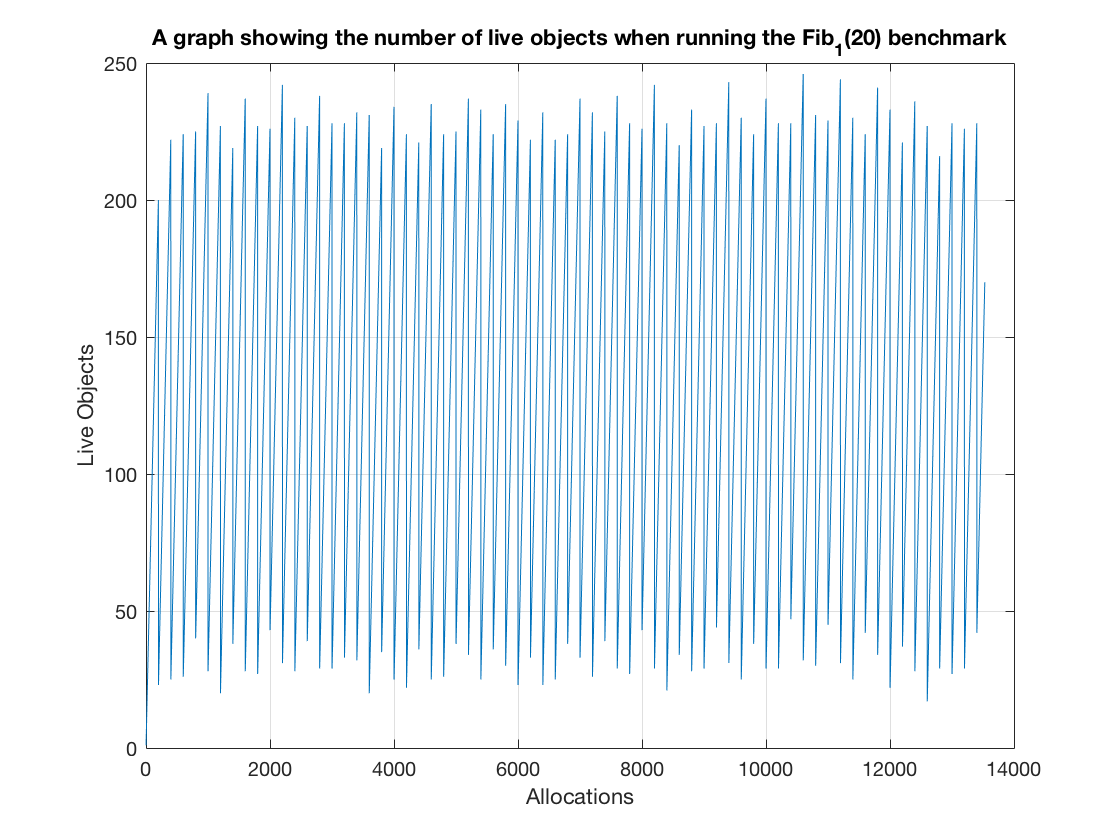
\includegraphics[max width=\linewidth]{figs/fib1.png}
    \caption{A figure showing how the number of live objects changes during runtime}
    \label{fig:fib1graph}
\end{figure}

\begin{table}
    \centering
    \begin{tabular}{| l | l |}
        \hline
         \bf{Statistic} & \bf{Result} \\ \hline
         Objects Allocated & 13529 \\ \hline
         Objects Freed & 13359 \\ \hline
         Total Collections & 67 \\ \hline
         Gen 0 Collections & 67 \\ \hline
         Gen 1 Collections & 44 \\ \hline
         Gen 2 Collections & 22 \\ \hline
    \end{tabular}
    \caption{Table of garbage collector statistics for Fib1(20)}
    \label{tab:fib1stats}
\end{table}

For the multi-threaded version, 8 threads will each compute the 20th Fibonacci number. The benchmark completed with the output of 6765, 8 times as we would expect. Figure \ref{fig:fibngraph} shows the results for running this benchmark and Table \ref{tab:fibnstats} shows the garbage collector statistics after completion. Again the object threshold was 200 objects, we can see in the graph that the decreases in live objects occur every 200 allocations. From the table of statistics we can see that 99\% of garbage was collected. We can see that the multi-threaded extension is working as intended.

\begin{table}
    \centering
    \begin{tabular}{| l | l |}
        \hline
         \bf{Statistic} & \bf{Result} \\ \hline
         Objects Allocated & 108232 \\ \hline
         Objects Freed & 107943 \\ \hline
         Total Collections & 541 \\ \hline
         Gen 0 Collections & 541 \\ \hline
         Gen 1 Collections & 360 \\ \hline
         Gen 2 Collections & 180 \\ \hline
    \end{tabular}
    \caption{Table of garbage collector statistics for FibN(20)}
    \label{tab:fibnstats}
\end{table}

\begin{figure}
    \centering
    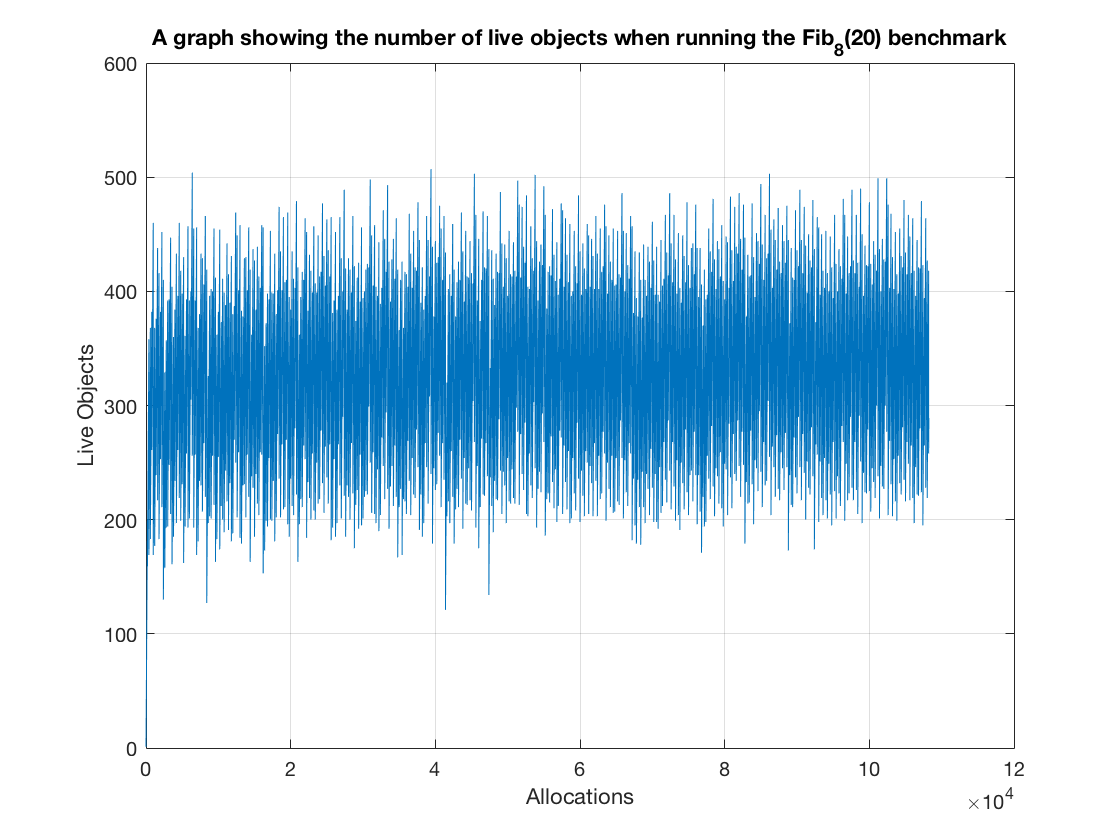
\includegraphics[max width=\linewidth]{figs/fib8.png}
    \caption{A figure showing how the number of live objects changes during runtime}
    \label{fig:fibngraph}
\end{figure}

We are also interested in the per-collection garbage collected. For this benchmark it is reasonable to say that 90\% of the objects created die quickly. We can assume this since every allocation is used to create intermediate values which get summed and discarded. Only the final result is not garbage but this is negligible. Figure \ref{fig:fibgarbagegraph} shows how the number of objects collected (frees) changes during runtime. On this graph I have plotted 90\% of the allocations as an approximation for the amount of garbage.

\begin{figure}
    \centering
    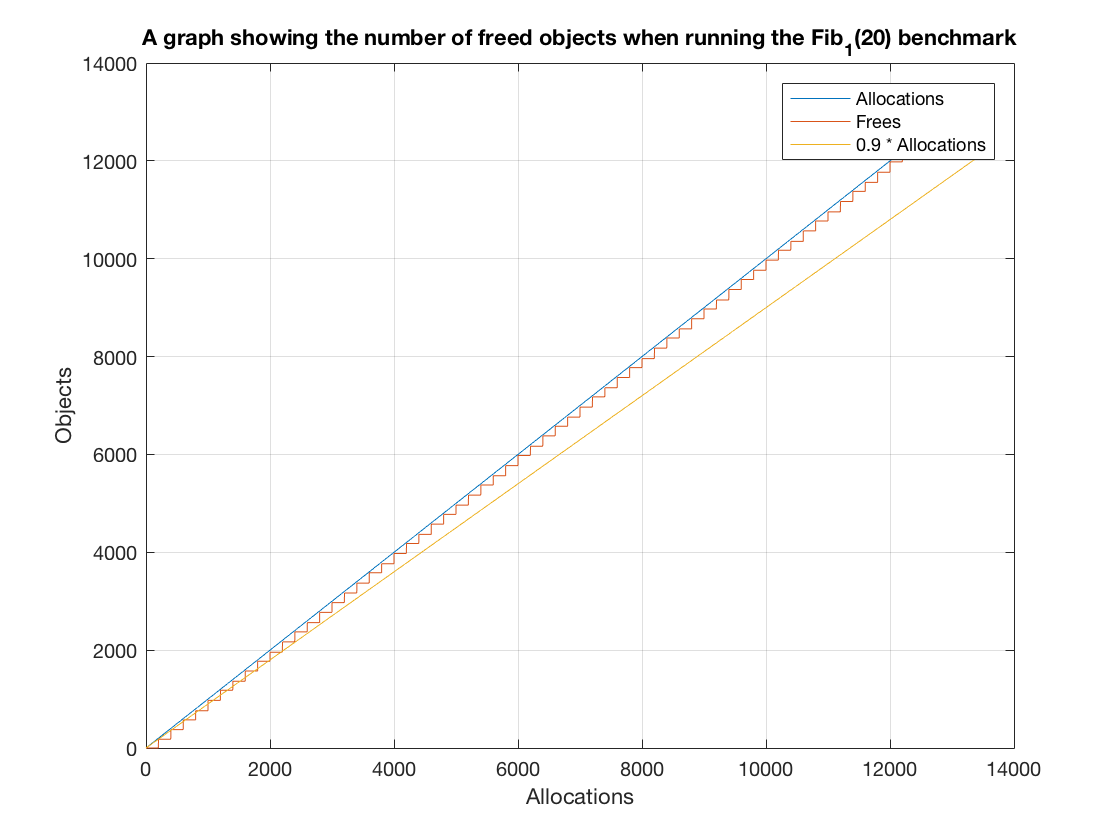
\includegraphics[max width=\linewidth]{figs/fibgarbage.png}
    \caption{A figure showing how much garbage is collected during runtime}
    \label{fig:fibgarbagegraph}
\end{figure}

\subsection{Trees Benchmark}

The trees benchmark simply produces a very large binary tree and then performs a traversal by counting the number of nodes. This benchmark allows us to verify that live objects are not collected in a convincing way, since the benchmark includes both object pointers and cross-generational pointers. Collecting a live object will cause the traversal to fail since the memory gets invalidated when freed. Table \ref{tab:trees1stats} shows the statistics for running this benchmark on a single thread with a threshold of 200 objects, from these we can see that no objects were collected. This is the desired result since the benchmark keeps the root node on the stack and therefore nothing is garbage.

\begin{table}
    \centering
    \begin{tabular}{| l | l |}
        \hline
         \bf{Statistic} & \bf{Result} \\ \hline
         Objects Allocated & 65535 \\ \hline
         Objects Freed & 0 \\ \hline
         Total Collections & 327 \\ \hline
         Gen 0 Collections & 327 \\ \hline
         Gen 1 Collections & 218 \\ \hline
         Gen 2 Collections & 109 \\ \hline
    \end{tabular}
    \caption{Table of garbage collector statistics for Trees1(16)}
    \label{tab:trees1stats}
\end{table}

The multi-threaded version simply produces 4 trees of height 16 over 4 different threads. The results can be seen in Table \ref{tab:treesnstats}. As we would expect none of the objects were freed and the results were correct.

\begin{table}
    \centering
    \begin{tabular}{| l | l |}
        \hline
         \bf{Statistic} & \bf{Result} \\ \hline
         Objects Allocated & 262140 \\ \hline
         Objects Freed & 0 \\ \hline
         Total Collections & 1310 \\ \hline
         Gen 0 Collections & 1310 \\ \hline
         Gen 1 Collections & 873 \\ \hline
         Gen 2 Collections & 436 \\ \hline
    \end{tabular}
    \caption{Table of garbage collector statistics for Trees4(16)}
    \label{tab:treesnstats}
\end{table}

% Describe the benchmarks, why they are used, the validity and the results

\section{Performance Evaluation}

In this section I will discuss how the threshold value impacts performance and how the overall performance (using the optimal parameters) compares with manual memory management. Despite not being a main success criterion it is important to discuss the impact on performance, as even in situations where this is not critical we still want to have minimal slowdown. All benchmarks are compiled with no optimisation to give worst-case runtime values.

\subsection{Variation with Threshold} \label{sec:variationwiththreshold}

The threshold is the number of allocations before the garbage collector runs. This value is fixed in the configuration and we see below how this impacts performance. Only the single threaded benchmarks are considered here for simplicity. 

The results of running the naive Fibonacci benchmark can be seen in Figure \ref{fig:fib_thresh}. This graph was produced by computing the 20th Fibonacci number and recording the runtime, 3 samples were taken for each threshold and a mean and standard deviation were calculated. The threshold was incremented each time by 500 up to a maximum of 5000. We can see from the results that the runtime does not vary significantly as the threshold changes. The reason for this is that the benchmark is designed to have almost every object die quickly. So as the threshold increases the garbage collector runs less frequently but at each collection there is more garbage to collect.

\begin{figure}
    \centering
    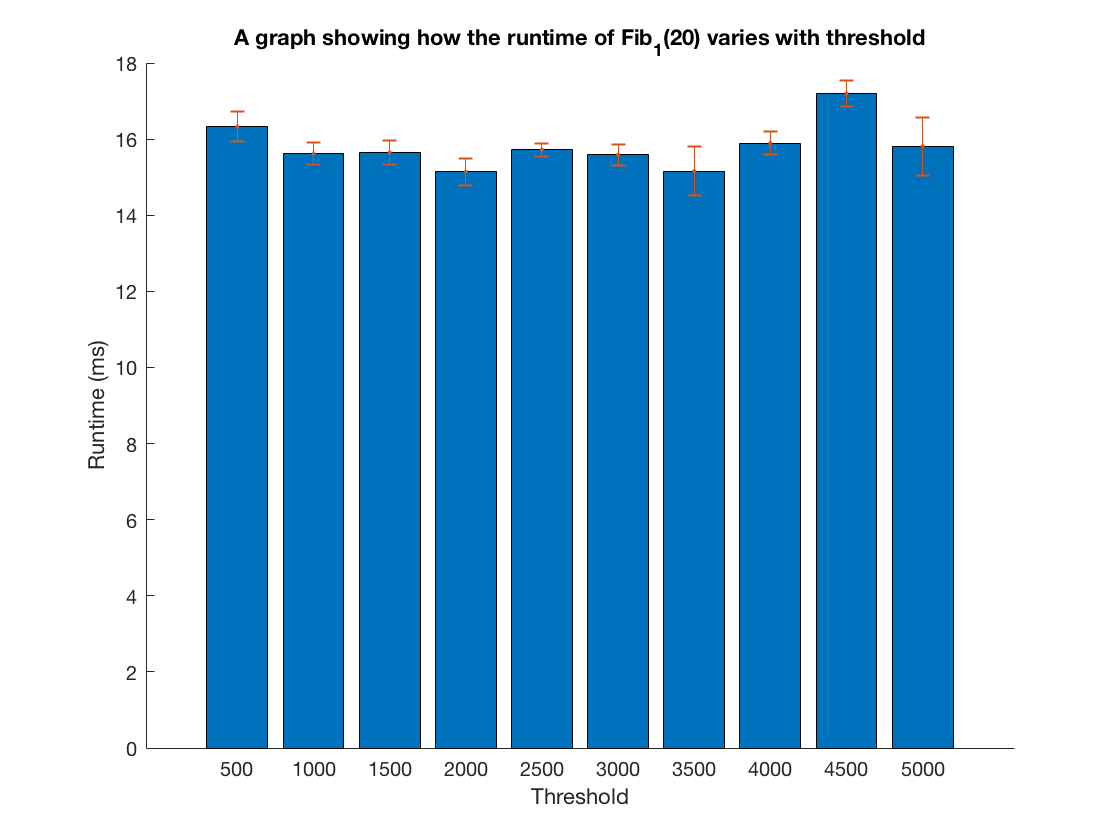
\includegraphics[max width=\linewidth]{figs/fib_threshold.png}
    \caption{A figure showing how the runtime of Fib1(20) varies with threshold}
    \label{fig:fib_thresh}
\end{figure}

The results of running the Trees benchmark can be seen in Figure \ref{fig:trees_thresh}. This graph was produced by building a tree of height 16. Table \ref{tab:trees1stats} shows the garbage collector stats for this benchmark. Again the increments in threshold are 500, but now up to a maximum of 10000 since the benchmark produces more objects than the naive Fibonacci. The results show that for small thresholds the runtime increases dramatically. This occurs because the Trees benchmark is does not produce any garbage. For small thresholds the garbage collector will run more frequently, but it will not remove any objects. Therefore, the search space never decreases with each collection and so collecting less frequently gives us better performance in this case. The best performance we can get for this benchmark is by choosing a threshold so large that the garbage collector never runs.

\begin{figure}
    \centering
    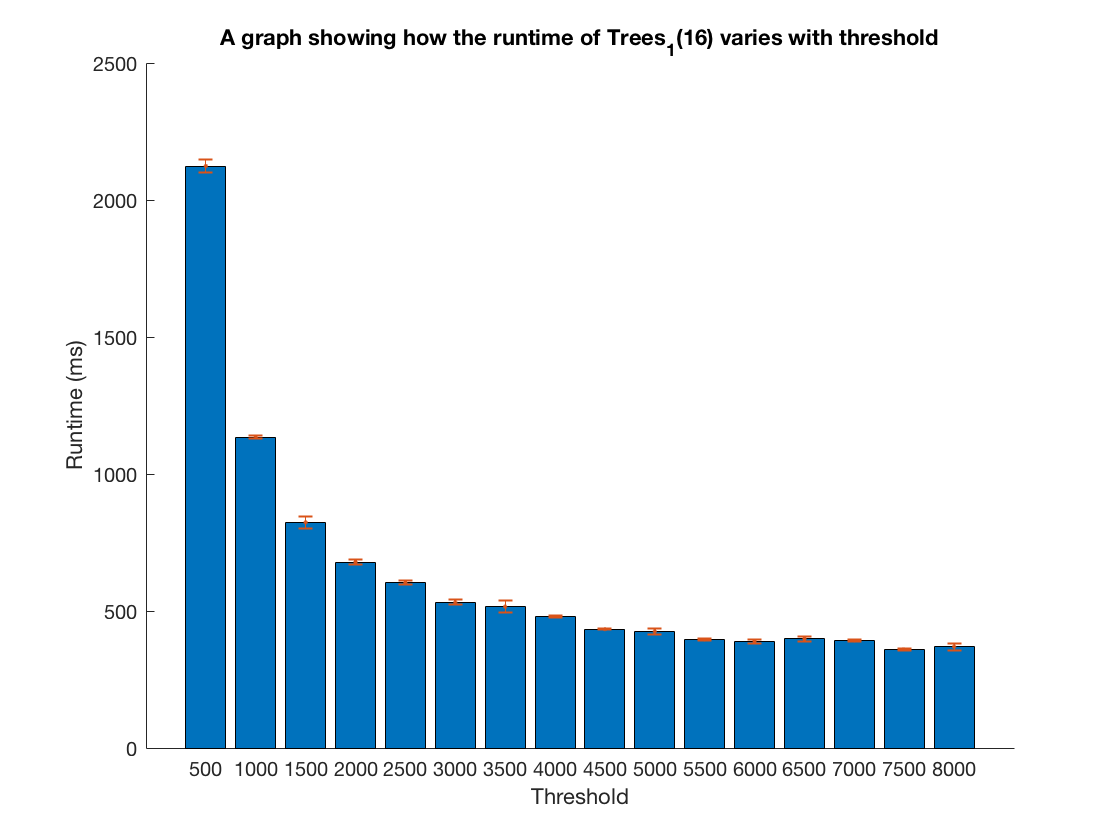
\includegraphics[max width=\linewidth]{figs/threes_thresh.png}
    \caption{A figure showing how the runtime of Trees1(16) varies with threshold}
    \label{fig:trees_thresh}
\end{figure}

It is clear that the choice of threshold and the type of workload can have a large impact on performance. By performing some form of static analysis an appropriate threshold can be chosen. A better solution would be to have a dynamic threshold which adjusts depending on the rate of allocations and the amount of garbage collected each time (see future work \cref{sec:futurework}).

\subsection{Comparison with Manual Memory Management}

A programmer that is interested in the garbage collector will be concerned with the best case performance hit. Comparing the two single-threaded benchmarks against the manual memory managed equivalents gives us a rough idea of the performance overhead. For each benchmark the optimal threshold is chosen using the evaluation from \cref{sec:variationwiththreshold}, with the requirement that it runs the garbage collector at least 5 times. As stated before we can get the best performance by simply making the threshold so large that the garbage collector never runs hence the extra condition.

Table \ref{tab:fibsamples} shows the samples made for the naive Fibonacci benchmark using a threshold of 2000 objects. Table \ref{tab:fibsummary} shows a summary of the results, from this we can see that the garbage collected version was $8.478 \pm 1.372\times$ slower.

\begin{table}
    \centering
    \begin{tabular}{| l | l |}
        \hline
         \multicolumn{2}{|c|}{\bf{Runtime / s}} \\ \hline
         \bf{MMM} & \bf{GC} \\ \hline
         0.001619 & 0.014706 \\ \hline
         0.001951 & 0.014529 \\ \hline
         0.001606 & 0.015088 \\ \hline
         0.001722 & 0.014583 \\ \hline
         0.001582 & 0.015543 \\ \hline
         0.001653 & 0.015008 \\ \hline
         0.001578 & 0.014657 \\ \hline
         0.002481 & 0.014609 \\ \hline
         0.001595 & 0.014791 \\ \hline
         0.001692 & 0.014674 \\ \hline
    \end{tabular}
    \caption{Table of runtime samples for Fib1(20)}
    \label{tab:fibsamples}
\end{table}

\begin{table}
    \centering
    \begin{tabular}{| l | l | l |}
        \hline
         & \bf{MMM} & \bf{GC} \\ \hline
         Average / s & 0.001748 & 0.01489 \\ \hline
         Standard Deviation / s & 0.0002805 & 0.0003122 \\ \hline
        
    \end{tabular}
    \caption{Summary of runtime results for Fib1(20)}
    \label{tab:fibsummary}
\end{table}

Table \ref{tab:treesamples} shows the samples made for the Trees benchmark using a threshold of 6000 objects. Table \ref{tab:treesummary} shows the results from these samples, from this we can see that the garbage collected version was $64.79 \pm 5.437\times$ slower.

Of the two benchmarks, naive Fibonacci is the more suitable for this type of garbage collector since the garbage assumptions hold. The Trees benchmark represents the type of data not well suited to generational garbage collection because every object is a long-lived one. 

When using the garbage collector, the programmer can improve performance by combining both manual memory management and automatic memory management, using the explicit malloc and free for long-lived data and using the \emph{GC\_malloc} for short-lived data.

\begin{table}
    \centering
    \begin{tabular}{| l | l |}
        \hline
         \multicolumn{2}{|c|}{\bf{Runtime / s}} \\ \hline
         \bf{MMM} & \bf{GC} \\ \hline
         0.006057 & 0.386979 \\ \hline
         0.00592 & 0.398611 \\ \hline
         0.005529 & 0.379001 \\ \hline
         0.005901 &	0.397257 \\ \hline
         0.006833 &	0.384114 \\ \hline
         0.005824 &	0.385439 \\ \hline
         0.005649 &	0.394008 \\ \hline
         0.005587 &	0.37599 \\ \hline
         0.005781 &	0.398424 \\ \hline
         0.006913 & 0.387119 \\ \hline
    \end{tabular}
    \caption{Table of runtime samples for Trees1(16)}
    \label{tab:treesamples}
\end{table}

\begin{table}
    \centering
    \begin{tabular}{| l | l | l |}
        \hline
         & \bf{MMM} & \bf{GC} \\ \hline
         Average / s & 0.005999 & 0.3887 \\ \hline
         Standard Deviation / s & 0.0004878 & 0.008075 \\ \hline
        
    \end{tabular}
    \caption{Summary of runtime results for Trees1(16)}
    \label{tab:treesummary}
\end{table}

\section{Summary}

In this chapter, I have provided evidence that the main success criteria have been met. This was achieved using two benchmarks which collectively display the robustness of the garbage collector, as well as multi-threaded versions which demonstrate that it's thread-safe. I have also discussed the performance of the garbage collector, showing how parameters can be changed to alter performance and how the memory characteristics of the program can have a large impact on the performance. These leads us to think differently about how C programs with garbage collection can be designed to minimise the performance hit.

\end{document}